\documentclass{article}
\usepackage[utf8]{inputenc}
\usepackage{lambdatex} %disponibile all'indirizzo http://lambdamath.altervista.it/esercizi/lambdatex.sty


\title{Università degli Studi di Trento - Dipartimento di Matematica\\
CdL in Matematica – a.a. 2022–2023\\ Note esercitazione}
\author{Esercitatore: Simone Verzellesi\thanks{Trascrizione a cura di Davide Borra}}
\date{19 Settembre 2022}

\begin{document}
\maketitle
\lhead{Note esercitazione}
\chead{Università degli Studi di Trento - Dipartimento di Matematica\\
CdL in Matematica – a.a. 2022–2023}
\rhead{19/09/2022}
\begin{enumerate}[label=\textbf{Esercizio 1.\arabic*.},itemindent=*]
    \item Dati i sottoinsiemi di $\R$:
    \begin{itemize}
        \item $A=\left\{\frac{1}{n}:n\in \N, n\neq 0\right\}$
        \item $B=[0,1[$
        \item $C=\Q$
        \item $D=\left\{0,\frac{1}{2},1\right\}$
    \end{itemize}
    Determinare $A\cap B$, $A\cap C$, $A\cup B$, $B^C$, $A\setminus B$,$A\triangle D$, $\mathcal{P}(D)$
    \item[\textit{\large Soluzione}]
    Sia $A'=A\setminus\{1\}$
    \begin{itemize}
        \item $A\cap B=A'$
        \item $A\cap C=A$, infatti se $P,R$ insiemi e $P\subseteq R$, allora $P\cap R=P$
        \item $A\cup B=[0,1]$
        \item $B^C=]-\infty,0[\cup[1,+\infty[$
        \item $A\setminus B=\{x\in A \land x \notin B\}=A\cap B^C=\{1\}$
        \item $A\triangle D=A\setminus D\cup D\setminus A=A\cup D \setminus A\cap D=\{0\}\cup \left\{\frac{1}{n}, n>0\right\}$
        \item $\mathcal{P}(D)=\{\varnothing, \{0\}, \{\frac{1}{2}\}, \{1\}, \{0, \frac{1}{2}\}, \{0,1\}, \{\frac{1}{2}, 1\}, D\}$
    \end{itemize}
    
    
    \item Rappresentare in $R^2$ i seguenti insiemi:
    \begin{itemize}
        \item $A=\{(x,y)\in \R^2:x+y\leq1\}$
        \item $B=\{(x,y)\in \R^2:|x|+|y|\leq 1\}$
        \item $C=\{(x,y)\in \R^2: |x|\leq 1\}$
        \item $D=\{(x,y)\in \R^2: y\leq 2x^2\}$
    \end{itemize}
    \item[\textit{\large Soluzione}]~
    \begin{figure}[h]
        \centering
        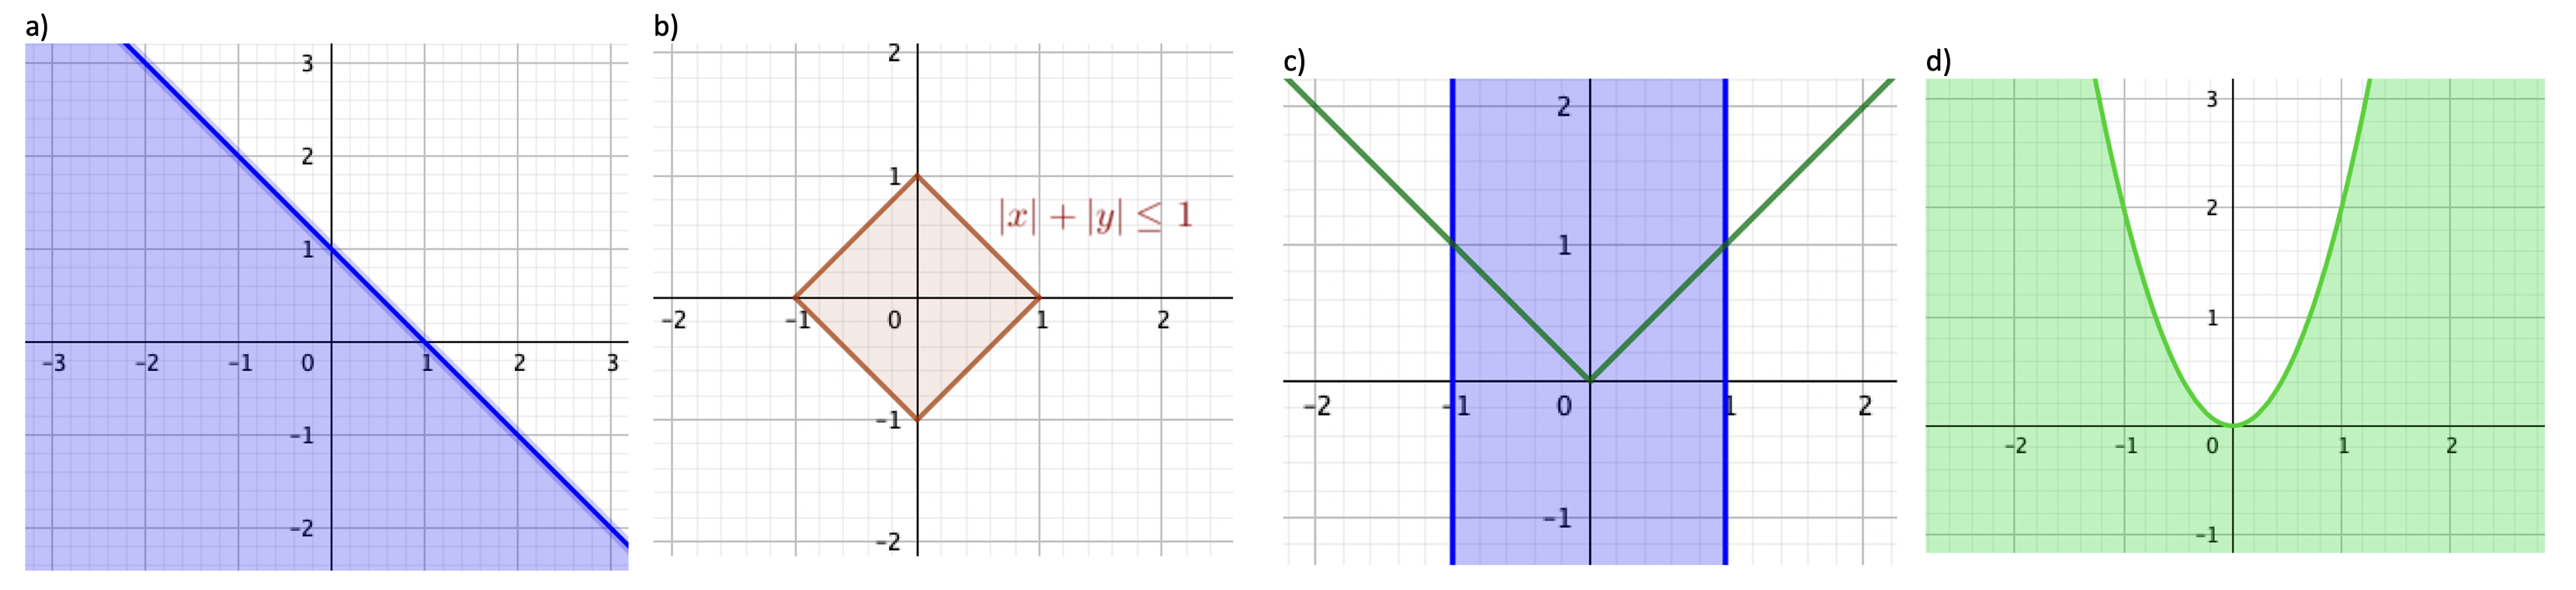
\includegraphics[width=0.9\textwidth]{Es2.png}
        %\caption{Caption}
        %\label{fig:my_label}
    \end{figure}
    \item Formalizzare e negare la seguente proprietà: \say{Esiste un numero naturale $n$ tale che per ogni numero naturale $z$ si ha che se $z$ è diverso da $n$, allora $z$ è minore di $n$}. Verificare se tale proprietà è vera o falsa.
    \item[\textit{\large Soluzione}]~ $\exists n\in \N :\forall z\in \N, z\neq \N\Rightarrow z<n~~~(F)$\\
    La negazione è $\forall n\in \N\exists z \in \N :z\neq n\land z\geq n~~~(V)$
    \item Data una proprietà $\mathcal{P}(x)$, formalizzare il fatto che esiste un unico $x$ che realizza $\mathcal{P}$ senza utilizzare il simbolo $\exists!$.
    \item[\textit{\large Soluzione~}]
    $\exists x:\mathcal{P}(x)\land \forall y,(y\neq x\Rightarrow\lnot \mathcal{P}(x))$
    \item Negare e stabilire la veridicità della proprietà: \[\forall x,y \in \R,(y>x\Rightarrow \exists n \in \N: n x>y)\]
    \item[\textit{\large Soluzione}]
    $\exists x,y \in \R:(y>x \land \forall n \in \N, nx\leq y)$
    \item Rappresentare il grafico della funzione $f(x)=\ln(|x-3|)$, dopo averne determinato il dominio.
    \item[\textit{\large Soluzione~}] Dominio: $|x-3|>0 \Leftrightarrow x\neq 3$
    \begin{figure}[h]
        \centering
        \definecolor{qqwuqq}{rgb}{0.,0.39215686274509803,0.}
        \begin{tikzpicture}[line cap=round,line join=round,>=triangle 45,x=1.0cm,y=1.0cm]
        \begin{axis}[
        x=0.8cm,y=0.8cm,
        axis lines=middle,
        ymajorgrids=true,
        xmajorgrids=true,
        xmin=-3.100000000000001,
        xmax=8.500000000000004,
        ymin=-3.3000000000000007,
        ymax=3.960000000000001,
        xtick={-3.0,-2.0,...,8.0},
        ytick={-3.0,-2.0,...,3.0},]
        \clip(-3.1,-3.3) rectangle (8.5,3.96);
        \draw[line width=2.pt,color=qqwuqq,smooth,samples=100,domain=-3.100000000000001:8.500000000000004] plot(\x,{ln(abs((\x)-3))});
        \end{axis}
        \end{tikzpicture}
    \end{figure}
    \item Rappresentare il grafico di $f_\alpha (x)=x^\alpha$, dopo averne determinato il dominio, con \[\alpha \in \N_{\geq 0} \cup \left\{\frac{1}{n}, n \in \N_{>0}\right\}\]. Discutere iniettività e suriettività di $f_\alpha$.
    \item[\textit{\large Soluzione~}] Se $\alpha \in \N \land \alpha \text{ pari}$ si tratta di una funzione potenza di grado pari, quindi né iniettiva né suriettiva. Se $\alpha$ dispari la funzione è una potenza di grado dispari, quindi sia iniettiva che suriettiva.\\
    Se $\alpha \in \left\{\frac{1}{n}, n \in \N_{>0}\right\}$, con $n$ pari, la funzione è una radice di indice pari, per cui è iniettiva ma non suriettiva. Se $n$ è dispari si tratta di una radice di indice dispari, quindi di una funzione iniettiva e suriettiva.
    \item Dimostrare che $f:\R\setminus \{0\}\to \R$ definita come \[f(x)=x+\frac{1}{x}\] non è iniettiva.
    \item[\textit{\large Soluzione~}] \begin{proof}$f(x)$ è iniettiva $\Leftrightarrow \forall x,y f(x)=f(y)\Rightarrow x=y$, quindi:
    \[x+\frac{1}{x}=y+\frac{1}{y}~~\Leftrightarrow~~x-y=\frac{1}{y}-\frac{1}{x}~~\Leftrightarrow~~x-y=\frac{x-y}{xy}\]
    Questa uguaglianza è verificata se e solo se $xy=1$, quindi non solo per $x=y$. Di conseguenza la funzione non è iniettiva.\end{proof}
\end{enumerate}
\end{document}
